
% v2-acmsmall-sample.tex, dated March 6 2012
% This is a sample file for ACM small trim journals
%
% Compilation using 'acmsmall.cls' - version 1.3 (March 2012), Aptara Inc.
% (c) 2010 Association for Computing Machinery (ACM)
%
% Questions/Suggestions/Feedback should be addressed to => "acmtexsupport@aptaracorp.com".
% Users can also go through the FAQs available on the journal's submission webpage.
%
% Steps to compile: latex, bibtex, latex latex
%
% For tracking purposes => this is v1.3 - March 2012
\documentclass[prodmode,acmtecs]{acmsmall} % Aptara syntax
\usepackage[spanish,polish]{babel}
\usepackage[T1]{fontenc}
\usepackage{fancyvrb}
\usepackage{graphicx,hyperref}
\newcommand\cutout[1]{}


\usepackage[table]{xcolor}
\usepackage[utf8]{inputenc}
\usepackage[parfill]{parskip}
\usepackage{tabulary}
\PassOptionsToPackage{hyphens}{url}
\usepackage{hyperref}    
\usepackage[capitalize]{cleveref}


% Metadata Information
% !!! TODO: SET THESE VALUES !!!
\acmVolume{0}
\acmNumber{0}
\acmArticle{CFP}
\acmYear{0}
\acmMonth{0}

\newcounter{colstart}
\setcounter{page}{4}

\RecustomVerbatimCommand{\VerbatimInput}{VerbatimInput}%
{
%fontsize=\footnotesize,
fontfamily=\rmdefault
}


\newcommand{\UnderscoreCommands}{%\do\verbatiminput%
\do\citeNP \do\citeA \do\citeANP \do\citeN \do\shortcite%
\do\shortciteNP \do\shortciteA \do\shortciteANP \do\shortciteN%
\do\citeyear \do\citeyearNP%
}

\usepackage[strings]{underscore}



% Document starts
\begin{document}


\setcounter{colstart}{\thepage}

\acmArticle{CFP}
\title{\huge\sc SIGLOG Monthly 227}
\author{DAVID PURSER\affil{University of Warsaw, Poland}
\vspace*{-2.6cm}\begin{flushright}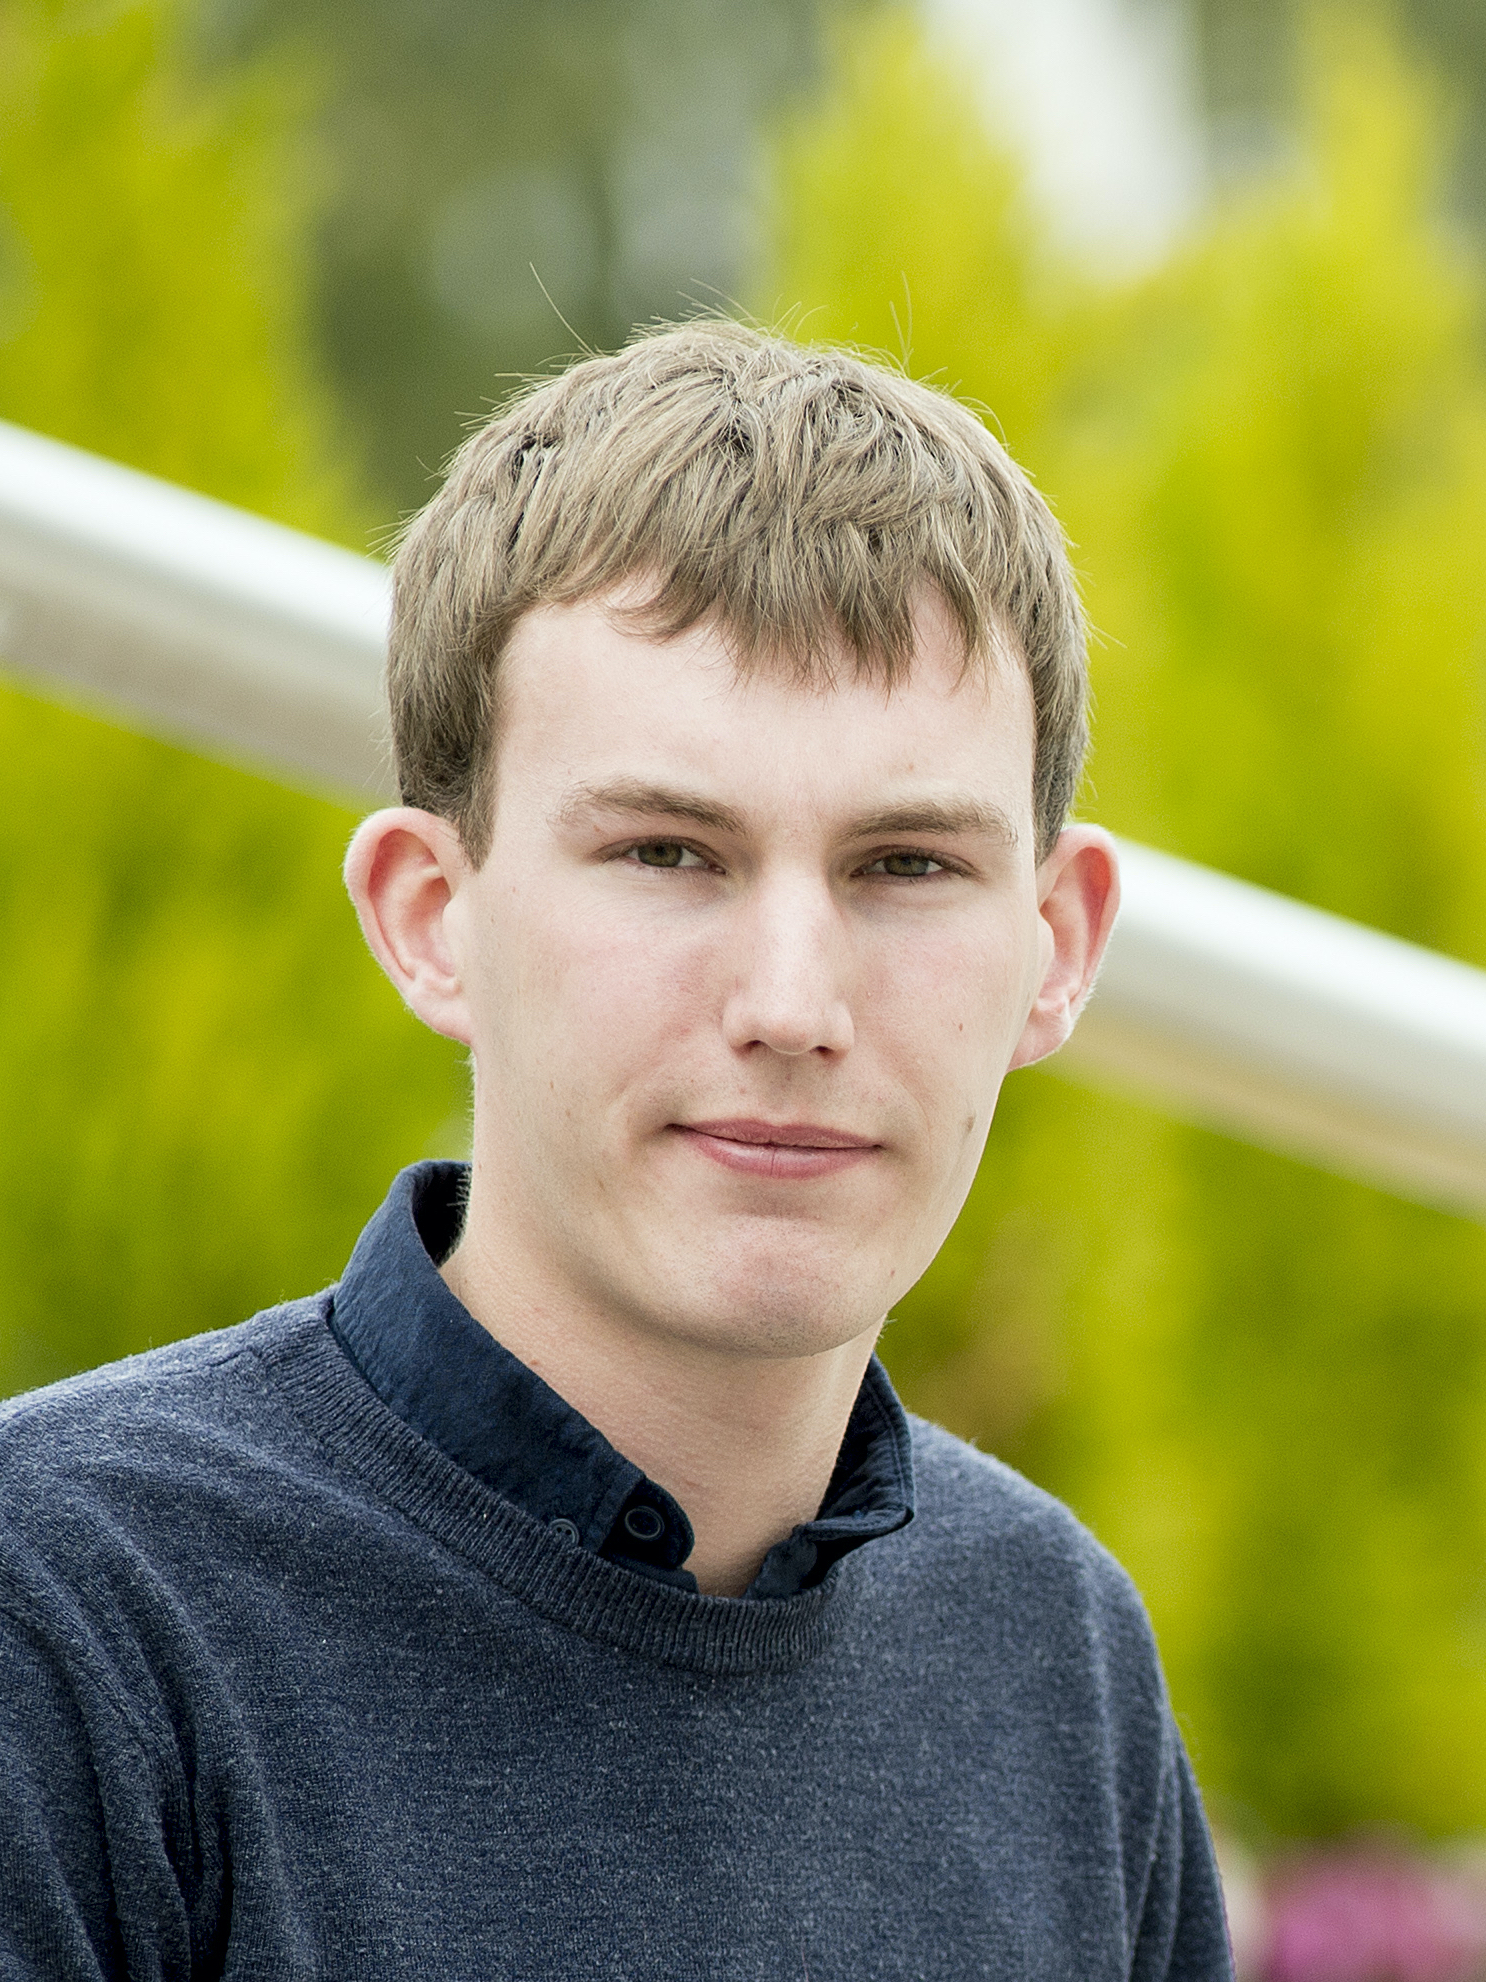
\includegraphics[width=30mm]{dp}\end{flushright}
}

\maketitlee

\href{https://lics.siglog.org/newsletters/}{Past Issues}
 - 
\href{https://lics.siglog.org/newsletters/inst.html}{How to submit an announcement}
\section{Table of Content}\begin{itemize}\item DEADLINES (\cref{deadlines}) 
 
\item SIGLOG MATTERS 
 
\begin{itemize}\item FLOC 2022 (\cref{FLOC2022})
\item ACM SIGLOG ELECTIONS ANNOUNCEMENT (\cref{ACMSIGLOGELECTIONSANNOUNCEMENT})
\item MFPS 2022 (\cref{MFPS2022})
\end{itemize} 
\item CALLS 
 
\begin{itemize}\item LearnAut 2022 (CALL FOR PARTICIPATION) (\cref{LearnAut2022})
\item LPNMR 2022 (CALL FOR PARTICIPATION) (\cref{LPNMR2022})
\item LPNMR Doctoral Consortium 2022 (CALL FOR CONTRIBUTIONS) (\cref{LPNMRDoctoralConsortium2022})
\item WiL 2022 (CALL FOR PARTICIPATION) (\cref{WiL2022})
\item DECFOML (CALL FOR PARTICIPATION) (\cref{DECFOML})
\item ASL 2022 (CALL FOR PARTICIPATION) (\cref{ASL2022})
\item ESSLLI 2022 (CALL FOR PARTICIPATION) (\cref{ESSLLI2022})
\item AiML 2022 (CALL FOR PARTICIPATION) (\cref{AiML2022})
\item CPP 2023 (CALL FOR PAPERS) (\cref{CPP2023})
\item OVERLAY 2022 (CALL FOR PAPERS) (\cref{OVERLAY2022})
\item FSEN 23 (CALL FOR PAPERS) (\cref{FSEN23})
\end{itemize} 
\item JOB ANNOUNCEMENTS 
 
\begin{itemize}\item POST-DOC POSITION IN LOGIC at LUCI-UNIMI (\cref{POSTDOCPOSITIONINLOGICatLUCIUNIMI})
\end{itemize} 
\end{itemize}\section{Deadlines}\label{deadlines}\rowcolors{1}{white}{gray!25}\begin{tabulary}{\linewidth}{LL}Datalog 2.0 2022:  & Jul 01, 2022 (Paper registration), Jul 08, 2022 (Paper) \\
ACKERMANN AWARD 2022:  & Jul 01, 2022 (Deadline for nomination) \\
LPNMR Doctoral Consortium 2022:  & Jul 06, 2022 (Application) \\
RCRA 2022:  & Jul 10, 2022 (Paper deadline) \\
FLOC 2022:  & Jul 20, 2022 (Regular registration closes) \\
LPNMR 2022:  & Jul 20, 2022 (Early registration deadline) \\
AiML 2022:  & Aug 10, 2022 (Registration deadline) \\
The ALP Alain Colmerauer Prolog Heritage Prize:  & Sep 02, 2022 (Deadline for nominations) \\
CPP 2023:  & Sep 14, 2022 (Abstract), Sep 21, 2022 (Paper) \\
OVERLAY 2022:  & Sep 30, 2022 (Paper) \\
FSEN 23:  & Oct 07, 2022 (Abstract), Oct 14, 2022 (Paper) \\
PODS 2023:  & Nov 28, 2022 (Second cycle abstract), Dec 05, 2022 (Full paper) \\
\end{tabulary}
\section{FLOC 2022: The Eighth Federated Logic Conference}\label{FLOC2022}  July 31-August 12, 2022, Haifa, Israel \\ 
  \href{https://www.floc2022.org/}{https://www.floc2022.org/}\\ 
CALL FOR PARTICIPATION 

\begin{itemize}\item  IMPORTANT INFORMATION 
 
Regular registration closes: Jul 20, 2022 
 
  ON-SITE REGISTRATION will be possible during the conference. 
 
  The conference will take place IN PERSON, see \href{https://www.floc2022.org/covid-19}{https://www.floc2022.org/covid-19} for the latest COVID regulations. 
 
  It is imperative that you BOOK ACCOMMODATION ASAP to avoid disappointment. 
 
\begin{itemize}\item  Registration: \href{https://www.floc2022.org/registration}{https://www.floc2022.org/registration}
\item  Accommodation: \href{https://www.floc2022.org/accommodation}{https://www.floc2022.org/accommodation}
\end{itemize} 
  Registration for the main conference block gives you access to any other conference in the same period. Conference registration includes reception, lunches, and coffee breaks. A banquet ticket can be added to the conference registration. 
 
  Registration for a workshop day means you can attend any other workshop on the same day. Workshop registration includes lunches and coffee breaks. 
 
\item  ACCOMMODATION 
 
  \href{https://www.floc2022.org/accommodation}{https://www.floc2022.org/accommodation} 
 
  We have made block bookings at several locations in Haifa until mid-May and any unsold rooms are now being released. It is imperative that you book NOW to avoid disappointment, as July/August is a busy period in Haifa! 
 
\item  ABOUT FLOC 
 
  During the past forty years there has been extensive, continuous, and growing interaction between logic and computer science. In many respects, logic provides computer science with both a unifying foundational framework and a tool for modeling. In fact, logic has been called “the calculus of computer science”, playing a crucial role in diverse areas such as artificial intelligence, computational complexity, distributed computing, database systems, hardware design, programming languages, and software engineering. 
 
  The Federated Logic Conference brings together several international conferences related to mathematical logic and computer science and was first organized in 1996, as part of the DIMACS Special Year on Logic and Algorithms. Since then FLoC was held in Trento in 1999, Copenhagen in 2002, Seattle in 2006, Edinburgh in 2010, Vienna in 2014, and Oxford in 2018. 
 
  The eighth Federated Logic Conference (FLoC'22) will be held in Haifa, Israel, in July 2022. 
 
\item  CONFERNCES 
 
  FLoC 2022 brings together twelve major international conferences, 70+ workshops, and several special events. 
 
\begin{itemize}\item  CAV \href{http://i-cav.org/2022/}{http://i-cav.org/2022/}
\item  CP \href{https://cp2022.a4cp.org/}{https://cp2022.a4cp.org/}
\item  CSF \href{https://www.ieee-security.org/TC/CSF2022/}{https://www.ieee-security.org/TC/CSF2022/}
\item  DL \href{https://dai.fmph.uniba.sk/events/dl2022/}{https://dai.fmph.uniba.sk/events/dl2022/}
\item  FSCD \href{https://www.cs.tau.ac.il/~nachumd/FSCD/}{https://www.cs.tau.ac.il/~nachumd/FSCD/}
\item  ICLP \href{https://software.imdea.org/Conferences/ICLP2022/}{https://software.imdea.org/Conferences/ICLP2022/}
\item  IJCAR \href{https://easychair.org/cfp/IJCAR-2022}{https://easychair.org/cfp/IJCAR-2022}
\item  ITP \href{https://itpconference.github.io/ITP22/}{https://itpconference.github.io/ITP22/}
\item  KR \href{https://kr2022.cs.tu-dortmund.de/}{https://kr2022.cs.tu-dortmund.de/}
\item  NMR \href{https://sites.google.com/view/nmr2022/home-page}{https://sites.google.com/view/nmr2022/home-page}
\item  LICS \href{https://lics.siglog.org/lics22/}{https://lics.siglog.org/lics22/}
\item  SAT \href{http://satisfiability.org/SAT22/}{http://satisfiability.org/SAT22/}
\end{itemize} 
\item  KEYNOTES/PLENARY LECTURES 
 
\begin{itemize}\item  Catuscia Palamidessi, Director of Research at INRIA
\item  Don Knuth, CP invited speaker, The Art of Computer Programming at Stanford University
\item  Orna Kupferman, School of Computer Science and Engineering at The Hebrew University of Jerusalem
\item  Ziyad Hanna, Corporate Vice President at Cadence Design Systems
\item  Aarti Gupta, Department of Computer Science at Princeton University
\end{itemize} 
\item  CONFERENCE INVITED SPEAKERS 
 
\begin{itemize}\item  CAV: Arie Gurfinkel, Neha Rungta
\item  FSCD: Cynthia Kop, Alwen Tiu
\item  ICLP: Fabrizio Riguzzi, Theresa Swift
\item  LICS: Amal Ahmed, Mikolaj Bojanczyk
\item  KR: Yejin Choi, Tony Hunter, Leonid Libkin
\end{itemize} 
\item  SOCIAL EVENTS 
 
  There is one Reception and one Banquet during each FLoC block, and one Workshop Dinner during each of the workshop blocks. For details, see \href{https://www.floc2022.org/program}{https://www.floc2022.org/program}. Guests are welcome: you can reserve your place(s) via the registration system. 
 
\item  SPECIAL EVENTS 
 
  Two logic lounges are held - one on August 2nd and the other on August 7th. See \href{https://www.floc2022.org/logiclounge}{https://www.floc2022.org/logiclounge} for details. 
 
\item  MENTORING WORKSHOPS 
 
  Two mentoring workshops will be held, on August 1 and August 5. 
 
  The purpose of the FLoC 2022 Mentoring Workshop (FLoC'22 MW) is to provide mentoring and career advice to early-stage graduate students, to attract them to pursue research careers in various logic-related areas. The workshop will particularly encourage participation of women and under-represented minorities. There will be two workshop days, one for each FLoC Conference Block, so the students can choose which one of the two they prefer to attend. The workshop program will include a number of talks and interactive sessions. Talks will give an overview of the field along with brief introductions to the varied topics highlighted at FLoC. Other talks will provide mentoring and career advice, from academia and industry.  
 
  Confirmed speakers: 
 
\begin{itemize}\item  Rajeev Alur, University of Pennsylvania, USA
\item  Nikolaj Bjorner, Microsoft Research, USA
\item  Liron Cohen, Ben-Gurion University, Israel
\item  Christoph Haase, University of Oxford, UK
\item  Kristin Rozier, Iowa State University, USA
\item  Neha Rungta, AWS, USA
\item  Natarajan Shankar, SRI, USA
\item  Alexandra Silva, Cornell University, USA
\end{itemize} 
  See \href{https://www.floc2022.org/flocmentoringworkshop}{https://www.floc2022.org/flocmentoringworkshop} for more details. 
 
\item  SPONSORSHIP 
 
  We are indebted to our sponsors for making FLoC possible, see: \href{https://www.floc2022.org/sponsors}{https://www.floc2022.org/sponsors} 
 
\item  LOCAL INFORMATION 
 
  Our website includes details for travel (including accessibility), venues, and things to do in Haifa for our attendees and their families: see \href{https://www.floc2022.org/information}{https://www.floc2022.org/information} for more information. 
 
  FLoC 2022 promises to be an exciting meeting, and we hope to see you in Haifa! 
 
\item  CALL FOR VOLUNTEERS 
 
  FLoC 2022 invites students to apply to our volunteer program. Volunteers will receive a stipend (a variable amount towards registration and travel costs for students depending on the origin of travel) in exchange for volunteer work at the conference. FLoC’22 volunteers will be able to interact with speakers and participants, network with other researchers, and meet graduate students from all over the world. See \href{https://www.floc2022.org/volunteers}{https://www.floc2022.org/volunteers} for details. 
 
\item  ADDITIONAL INFORMATION 
 
  See \href{https://www.floc2022.org/about}{https://www.floc2022.org/about} 
 
\end{itemize}\section{ACM SIGLOG ELECTIONS ANNOUNCEMENT}\label{ACMSIGLOGELECTIONSANNOUNCEMENT}  \href{http://siglog.acm.org}{http://siglog.acm.org}\\ 
  \href{https://www.acm.org/elections/sigs/2022-sig-election/siglog-2022-results}{https://www.acm.org/elections/sigs/2022-sig-election/siglog-2022-results}\\ 
ANNOUNCEMENT 

\begin{itemize}\item  We are pleased to announce the 2022 ACM SIGLOG election results for the term of 1 July 2022 – 30 June 2025. The new SIGLOG Chair is Catuscia Palamidessi and the other officers are Andrzej Murawski (Vice-Chair), Elaine Pimentel (Treasurer) and Sandra Alves (Secretary). 
 
\item  In 2014, the ACM chartered a Special Interest Group on Logic and Computation (ACM SIGLOG). One can join SIGLOG by visiting \href{https://campus.acm.org/public/qj/gensigqj/siglist/gensigqj_siglist.cfm}{https://campus.acm.org/public/qj/gensigqj/siglist/gensigqj\_siglist.cfm}  
 
  It is possible to join SIGLOG without joining ACM (the SIGLOG membership fee is $25 and $15 for students). 
 
\end{itemize}\section{MFPS 2022: International Conference on Mathematical Foundations of Programming Semantics}\label{MFPS2022}  July 11-13, 2022\\ 
  Ithaca, NY + Paris + Online\\ 
  \href{https://www.cs.cornell.edu/mfps-2022/}{https://www.cs.cornell.edu/mfps-2022/}\\ 
CALL FOR PARTICIPATION 

\begin{itemize}\item  MFPS 38 will be held on July 11-13, 2022. We plan to hold a hybrid conference with the in-person event at Cornell University in Ithaca, New York, and an in-person local event in Paris, France.  
 
\item  REGISTRATION 
 
  \href{https://www.cs.cornell.edu/mfps-2022/#registrationandaccommodations}{https://www.cs.cornell.edu/mfps-2022/\#registrationandaccommodations} 
 
\end{itemize}\section{LearnAut 2022: The 4th workshop on Learning \& Automata - satellite of ICALP’22}\label{LearnAut2022}  \href{https://learnaut22.github.io/}{https://learnaut22.github.io/} \\ 
  July 4 2022, Paris \& on-line\\ 
CALL FOR PARTICIPATION 

\begin{itemize}\item  Location: building Halle aux Farines located in the heart of the site “Grands Moulins” of the Université de Paris.  
 
  This event will be conducted in hybrid mode: in person in Paris (organizers' preferred choice) and virtually. Registration is mandatory for both modes (please find the corresponding links here: \href{https://learnaut22.github.io/registration.html}{https://learnaut22.github.io/registration.html}) 
 
  It is our pleasure to inform you about LearnAut 2022, the fourth edition of the workshop, this time co-located with ICALP.  
 
  Learning models defining recursive computations, like automata and formal grammars, are the core of the field called Grammatical Inference (GI). The expressive power of these models and the complexity of the associated computational problems are major research topics within mathematical logic and computer science. Historically, there has been little interaction between the GI and ICALP communities, though recently some important results started to bridge the gap between both worlds, including applications of learning to formal verification and model checking, and (co-)algebraic formulations of automata and grammar learning algorithms. 
 
  The goal of this workshop is to bring together experts on logic who could benefit from grammatical inference tools, and researchers in grammatical inference who could find in logic and verification new fruitful applications for their methods. 
 
  The LearnAut workshop will consist of 3 invited talks and 14 contributed talks from researchers whose submitted works were selected after a double blind peer-reviewed phase. An important amount of time will be kept for interactions between participants. 
 
\item  Invited Speakers 
 
\begin{itemize}\item  Jeffrey Heinz, Stony Brook University, USA
\item  Sheila McIlraith, University of Toronto, Canada
\item  Ariadna Quattoni, Universitat Politècnica de Catalunya, Spain
\end{itemize} 
\end{itemize}\section{LPNMR 2022: 16th International Conference on Logic Programming and Non-monotonic Reasoning}\label{LPNMR2022}  \href{https://sites.google.com/view/lpnmr2022/}{https://sites.google.com/view/lpnmr2022/}\\ 
  Genova, Italy September 5-9, 2022\\ 
  \href{https://lpnmr2022.dibris.unige.it}{https://lpnmr2022.dibris.unige.it}\\ 
CALL FOR PARTICIPATION 

\begin{itemize}\item  REGISTRATION  
 
Early registration deadline: Jul 20, 2022 
 
  For more information, visit: \href{https://sites.google.com/view/lpnmr2022/registration}{https://sites.google.com/view/lpnmr2022/registration}  We remind that at least one author of each accepted paper must early register in order to have the paper included in the proceedings. 
 
\item  AIMS AND SCOPE 
 
  LPNMR 2022 is the sixteenth in the series of international meetings on logic programming and non-monotonic reasoning. LPNMR is a forum for exchanging ideas on declarative logic programming, non-monotonic reasoning, and knowledge representation. The aim of the conference is to facilitate interactions between researchers and practitioners interested in the design and implementation of logic-based programming languages and database systems, and those working in knowledge representation and non-monotonic reasoning. LPNMR strives to encompass theoretical and experimental studies that have led or will lead to advances in declarative programming and knowledge representation, as well as their use in practical applications. A Doctoral Consortium will also be a part of the program. 
 
  LPNMR 2022 aims to bring together researchers from LPNMR core areas and application areas of the aforementioned kind in order to share research experiences, promote collaboration and identify directions for joint future research.  
 
\item  VENUE 
 
  The main conference will take place in Genova Nervi, Italy, in the Collegio Emiliani (\href{http://www.collegioemiliani.it/}{http://www.collegioemiliani.it/} (in Italian)), which is a college directly situated on the sea. Nervi is a former fishing village, now a suburb of Genoa. Nervi is 7 km east of central Genova. Genova is the capital of Liguria, stretching along the bay of the same name from Nervi to the east as far as Voltri to the west. The pride of Nervi is the sea promenade, a 2 km walkway along the cliffs. The stunning views make it one of Italy's most beautiful promenades. Nervi is also well known for its Parchi, a park of about 22 acres (9 hectares) created from the gardens of the Villa Grimaldi, Villa Groppallo, and Villa Serra. It has typical Mediterranean plant species and many exotic species. Genova's old town district (reachable by local train, by bus, as well as by boat) is one of the largest in Europe, and hosts some remarkable artistic and architectural treasures, including the Palazzi dei Rolli, fifty or so homes of the aristocracy entered on the UNESCO World Heritage List. In addition to offering a wealth of cultural attractions, Genova is a fascinating destination for tourists, with its scenic vantage points, sea promenades, aristocratic villas and of course the Riviera to the east and west, both easy to reach: Portovenere and Le Cinque Terre (also UNESCO World Heritage Sites), Portofino and Camogli to the east and Alassio, Sanremo, Bordighera to the west. 
 
  Workshops and associated events, differently from what we mentioned in the previous call, are planned to be held in the main conference venue as well.  
 
  Of course, we will continuously monitor the pandemic situation in order to evaluate whether the conference can be indeed held as an in-person event, or we will need to switch to a hybrid event, if not completely on-line.  
 
\end{itemize}\section{LPNMR Doctoral Consortium 2022}\label{LPNMRDoctoralConsortium2022}  Genova, Italy\\ 
  September 5-8, 2022\\ 
  \href{https://sites.google.com/view/lpnmr2022/doctoral-consortium}{https://sites.google.com/view/lpnmr2022/doctoral-consortium}\\ 
CALL FOR CONTRIBUTIONS 

\begin{itemize}\item  TOPIC AND OBJECTIVE  
 
  The LPNMR Doctoral Consortium (DC) is to be held as part of the 16th International Conference on Logic Programming and Non-monotonic Reasoning (LPNMR 2022) in Genova, Italy, September 5-8, 2022. The DC provides a forum for doctoral students working in all areas related to logic programming and non-monotonic reasoning. The DC gives students the opportunity to present and discuss their research and to obtain feedback from peers as well as world-renowned experts in a supportive environment. 
 
  The 16th International Conference on Logic Programming and Non-monotonic Reasoning (LPNMR) is a forum for exchanging ideas on declarative logic programming, non-monotonic reasoning, and knowledge representation. The aim of the conference is to facilitate interactions between researchers and practitioners interested in the design, implementation and application of logic-based programming languages and database systems, and those who work in the area of knowledge representation and non-monotonic reasoning. 
 
  During the DC, there will be significant time for students to present their work, and meet mentors from their own and closely related fields. 
 
\item  TARGET AUDIENCE 
 
  The DC is designed for students currently enrolled in a PhD program, though we are also open to exceptions (e.g., students currently in a masters program and interested in doctoral studies). Students at any stage in their doctoral studies are encouraged to apply for participation in the DC, but preference will be given to students who have settled on a research topic or direction but still have some way to go in their studies. Applicants are expected to conduct research in areas related to logic and constraint programming; topics of interest include (but are not limited to): 
 
\begin{itemize}\item  Theoretical Foundations of LPNMR systems, including semantics of new or existing languages, new language extensions, and computational complexity
\item  Implementation of LPNMR systems, including new systems and algorithms
\item  Applications of LPNMR
\end{itemize} 
   The DC allows participants to interact with established researchers and fellow students, through presentations, a poster session, question-answer sessions and social interactions. The Doctoral Consortium will provide the possibility to reflect - through short activities, information sessions, and discussions - on the process and lessons of research and life in academia. Each participant will give a short, critiqued research presentation, present a poster at the main event and attend a lunch in small groups with their mentor/senior researcher. 
 
\item  APPLICATION PROCESS 
 
   Please see the full call for the application process: \href{https://sites.google.com/view/lpnmr2022/call-for/dc}{https://sites.google.com/view/lpnmr2022/call-for/dc} 
 
\item  IMPORTANT DATES 
 
\rowcolors{1}{white}{gray!25}\begin{tabulary}{\linewidth}{LL}Application submission:  & Jul 06, 2022 \\
Notification:  & Jul 20, 2022 \\
Camera-ready Version:  & Aug 10, 2022 \\
Doctoral Consortium (tentative):  & Sep 05, 2022 \\
\end{tabulary}
 
\end{itemize}\section{WiL 2022: 6th Women in Logic Workshop}\label{WiL2022}  July 31, 2022 part of FLoC 2022\\ 
  \href{https://sites.google.com/g.uporto.pt/wil2022}{https://sites.google.com/g.uporto.pt/wil2022}\\ 
  Note FLOC registration deadline\\ 
CALL FOR PARTICIPATION 

\begin{itemize}\item  Are you a woman working in logic? Please join us on July 31 at WiL, give a talk, and enjoy a day with Women in Logic! 
 
\item  Women in Logic 2022 is a satellite event of the 8th Federated Logic Conference (FLoC 2022) to be held in Haifa, Israel, from July 31 to August 12, 2022. The Women in Logic workshop (WiL) provides an opportunity to increase awareness of the valuable contributions made by women in the area of logic in computer science. Its main purpose is to promote the excellent research done by women, with the ultimate goal of increasing their visibility and representation in the community. Our aim is to: 
 
\begin{itemize}\item  provide a platform for female researchers to share their work and achievements;
\item  increase the feelings of community and belonging, especially among junior faculty, post-docs, and students through positive interactions with peers and more established faculty;
\item  establish new connections and collaborations;
\item  foster a welcoming culture of mutual support and growth within the logic research community. 
\end{itemize} 
  We believe these aspects will benefit women working in logic and computer science, particularly early-career researchers. Previous versions of Women in Logic (Reykjavík 2017, Oxford 2018, Vancouver 2019, Paris 2020, and Rome 2021) were very successful in showcasing women's work and as catalysts for a recognition of the need for change in the community. Topics of interest include but are not limited to: automata theory, automated deduction, categorical models and logics, concurrency and distributed computation, constraint programming, constructive mathematics, database theory, decision procedures, description logics, domain theory, finite model theory, formal aspects of program analysis, formal methods, foundations of computability, games and logic, higher-order logic, lambda and combinatory calculi, linear logic, logic in artificial intelligence, logic programming, logical aspects of bioinformatics, logical aspects of computational complexity, logical aspects of quantum computation, logical frameworks, logics of programs, modal and temporal logics, model checking, probabilistic systems, process calculi, programming language semantics, proof theory, real-time systems, reasoning about security and privacy, rewriting, type systems and type theory, and verification.  
 
\item  INVITED SPEAKERS 
 
\begin{itemize}\item  Dana Fisman (Ben-Gurion University of the Negev)
\item  Delia Kesner (IRIF - Université de Paris)
\end{itemize} 
\end{itemize}\section{DECFOML: LICS 2022 Affiliated Workshop on Decidable Fragments of First-order Modal Logic}\label{DECFOML}  \href{http://wangyanjing.com/decfoml}{http://wangyanjing.com/decfoml}\\ 
  31 July 2022, Haifa, Israel, Part of FLoC 2022 (\href{https://floc2022.org}{https://floc2022.org})\\ 
  Note FLOC registration deadline\\ 
CALL FOR PARTICIPATION 

  First-order modal logic is a natural specification language for describing properties of infinite-state systems, databases and de re knowledge of agents, but it is notoriously undecidable, in the sense that even simple fragments (like the two-variable fragment with unary predicates) are undecidable. Despite this, in the recent few years, researchers have managed to find some useful syntactic restrictions that yield decidability, such as monodic fragments and bundled fragments.\\ 
  The workshop is intended as a review of this rapidly evolving direction of research. We seek to identify new potential techniques for constructing decision procedures and discuss problem areas, in terms of syntactic restrictions as well as model classes.\\ 
\begin{itemize}\item  Invited Speakers: 
 
\begin{itemize}\item  Eugenio Orlandelli (University of Bologna) 
\item  Ian Pratt-Hartmann (University of Manchester) 
\item  Frank Wolter (University of Liverpool)
\end{itemize} 
\item  To register for the workshop: \href{https://www.floc2022.org/registration}{https://www.floc2022.org/registration} (You need not register for the conference as well.) 
 
\end{itemize}\section{ASL 2022: Workshop on Advances in Separation Logics }\label{ASL2022}  Haifa, Israel, July 31st 2022,  affiliated to IJCAR 2022, part of FLoC 2022 (\href{https://floc2022.org}{https://floc2022.org})\\ 
  \href{https://asl-workshop.github.io/asl22/}{https://asl-workshop.github.io/asl22/}\\ 
  Program:  \href{https://easychair.org/smart-program/FLoC2022/ASL-index.html}{https://easychair.org/smart-program/FLoC2022/ASL-index.html}\\ 
CALL FOR PARTICIPATION 

\begin{itemize}\item  REGISTRATION 
 
  In-person registration is done via the FLOC 2022 registration. Note FLOC registration deadline. 
 
  Virtual participation is free of charge but requires registration via the following link: \href{https://asl2022.rsvpify.com/}{https://asl2022.rsvpify.com/} 
 
\item  KEYNOTE SPEAKERS 
 
\begin{itemize}\item  Philippa Gardner, Imperial College London
\item  Ralf Jung, MIT CSAIL
\end{itemize} 
\end{itemize}\section{ESSLLI 2022: 33rd European Summer School on Logic, Language and Information.}\label{ESSLLI2022}  August 8-19, 2022, Galway, Ireland\\ 
  \href{https://2022.esslli.eu/}{https://2022.esslli.eu/}\\ 
CALL FOR PARTICIPATION 

\begin{itemize}\item   Registration is now open for the 33rd European Summer School in Logic, Language and Information (ESSLLI), taking place from 8-19 August, 2022 at the National University of Ireland Galway: \href{https://2022.esslli.eu/}{https://2022.esslli.eu/} 
 
\item  OVERVIEW 
 
  Registration is open for ESSLLI 2022, which will take place from August 8 to August 19, 2022 at The National University of Ireland Galway. ESSLLI is an annual event organised under the auspices of the Association for Logic, Language and Information (FoLLI). ESSLLI 2022 offers an exciting two-week programme, consisting of the following: 
 
\begin{itemize}\item  Workshops in logic, linguistics, and computer science
\item  Courses at three different levels (foundational, introductory, advanced) and in three areas: Language and Computation; Logic and Computation; Logic and Language.
\item  Student session
\item  Evening lectures by distinguished researchers
\item  Social activities.
\end{itemize} 
\item  Detailed information can be found at the website \href{https://2022.esslli.eu/}{https://2022.esslli.eu/} 
 
\end{itemize}\section{AiML 2022: 14TH INTERNATIONAL CONFERENCE ON ADVANCES IN MODAL LOGIC}\label{AiML2022}  Rennes, August 22-25, 2022\\ 
  Registration open until August 10, 2022\\ 
CALL FOR PARTICIPATION 

  Advances in Modal Logic is an initiative aimed at presenting the state of the art in modal logic and its various applications. The initiative consists of a conference series together with volumes based on the conferences.\\ 
  AiML 2022 will be co-located with the Workshop on Logical Aspects of Multi-Agent Systems and Strategic Reasoning (LAMAS\&SR 2022). \\ 
\begin{itemize}\item  REGISTRATION LINK 
 
Registration deadline: Aug 10, 2022 
 
  Please visit \href{https://aiml2022.irisa.fr/registration/}{https://aiml2022.irisa.fr/registration/} 
 
\item  WEBPAGES  
 
  AiML 2022: \href{http://www.aiml.net}{http://www.aiml.net} 
 
  AiML Series: \href{https://aiml2022.irisa.fr/}{https://aiml2022.irisa.fr/} 
 
  LAMAS\&SR: \href{https://lamassr.github.io/}{https://lamassr.github.io/} 
 
\item  TOPICS 
 
\begin{itemize}\item  history of modal logic
\item  philosophy of modal logic
\item  applications of modal logic
\item  computational aspects of modal logic
\item  theoretical aspects of modal logic
\item  specific instances and variations of modal logic
\end{itemize} 
\item  INVITED SPEAKERS 
 
\begin{itemize}\item  Willem Conradie, University of the Witwatersrand 
\item  Wesley Holliday, University of California, Berkeley 
\item  Francesca Poggiolesi, Sorbonne and CNRS 
\item  Rineke Verbrugge, University of Groningen (joint LAMAS\&SR speaker)
\end{itemize} 
\end{itemize}\section{CPP 2023: Certified Programs and Proofs}\label{CPP2023}  January 16-17, 2023 \\ 
  Boston, United States\\ 
  \href{https://popl23.sigplan.org/home/CPP-2023#Call-for-Papers}{https://popl23.sigplan.org/home/CPP-2023\#Call-for-Papers}\\ 
CALL FOR PAPERS 

\begin{itemize}\item  Certified Programs and Proofs (CPP) is an international conference on practical and theoretical topics in all areas that consider formal verification and certification as an essential paradigm for their work. CPP spans areas of computer science, mathematics, logic, and education. 
 
  CPP 2023 (\href{https://popl23.sigplan.org/home/CPP-2023}{https://popl23.sigplan.org/home/CPP-2023}) will be held on 16-17 January 2023 and will be co-located with POPL 2023 in Boston, Massachusetts, United States. CPP 2023 is sponsored by ACM SIGPLAN, in cooperation with ACM SIGLOG. 
 
  CPP 2023 will welcome contributions from all members of the community. The CPP 2023 organizers will strive to enable both in-person and remote participation, in cooperation with the POPL 2023 organizers. 
 
\item  IMPORTANT DATES (Strict, AoE) 
 
\rowcolors{1}{white}{gray!25}\begin{tabulary}{\linewidth}{LL}Abstract submission:  & Sep 14, 2022 \\
Paper submission:  & Sep 21, 2022 \\
Notification (tentative):  & Nov 21, 2022 \\
Camera Ready Deadline (tentative):  & Dec 12, 2022 \\
Conference:  & Jan 16-17, 2023 \\
\end{tabulary}
 
\item  DISTINGUISHED PAPER AWARDS 
 
  Around 10% of the accepted papers at CPP 2023 will be designated as Distinguished Papers. This award highlights papers that the CPP program committee thinks should be read by a broad audience due to their relevance, originality, significance and clarity. 
 
\item  TOPICS OF INTEREST 
 
  We welcome submissions in research areas related to formal certification of programs and proofs. The following is a non-exhaustive list of topics of interest to CPP: 
 
\begin{itemize}\item certified or certifying programming, compilation, linking, OS kernels, runtime systems, security monitors, and hardware; 
\item certified mathematical libraries and mathematical theorems; 
\item proof assistants (e.g, ACL2, Agda, Coq, Dafny, F*, HOL4, HOL Light, Idris, Isabelle, Lean, Mizar, Nuprl, PVS, etc); 
\item new languages and tools for certified programming; 
\item program analysis, program verification, and program synthesis; 
\item program logics, type systems, and semantics for certified code; 
\item logics for certifying concurrent and distributed systems; 
\item mechanized metatheory, formalized programming language semantics, and logical frameworks; 
\item higher-order logics, dependent type theory, proof theory, logical systems, separation logics, and logics for security; 
\item verification of correctness and security properties; 
\item formally verified blockchains and smart contracts; 
\item certificates for decision procedures, including linear algebra, polynomial systems, SAT, SMT, and unification in algebras of interest; 
\item certificates for semi-decision procedures, including equality, first-order logic, and higher-order unification; 
\item certificates for program termination; 
\item formal models of computation; 
\item mechanized (un)decidability and computational complexity proofs; 
\item formally certified methods for induction and coinduction; 
\item integration of interactive and automated provers; 
\item logical foundations of proof assistants; 
\item applications of AI and machine learning to formal certification; 
\item user interfaces for proof assistants and theorem provers; 
\item teaching mathematics and computer science with proof assistants.
\end{itemize} 
\item  SUBMISSION GUIDELINES 
 
  Please see the full call for comprehensive information about submission guidelines, publication, copyright and open access. 
 
\end{itemize}\section{OVERLAY 2022}\label{OVERLAY2022}  November 28-December 4, 2022 (the precise day(s) will be announced later)\\ 
  Udine, Italy (unless held online, depending on the pandemic emergency situation)\\ 
  \href{https://overlay.uniud.it/workshop/2022}{https://overlay.uniud.it/workshop/2022}\\ 
  Co-located with AIxIA 2022\\ 
  \href{https://aixia2022.uniud.it}{https://aixia2022.uniud.it}\\ 
CALL FOR PAPERS 

\begin{itemize}\item  The increasing adoption of Artificial Intelligence techniques in safety-critical systems, employed in real world scenarios, requires the design of reliable, robust, and verifiable methodologies. Artificial Intelligence systems employed in such applications need to provide formal guarantees about their safety, increasing the need for a close interaction between the Artificial Intelligence and Formal Methods scientific communities. 
 
  To witness this increasing need, tools and methodologies integrating Formal Methods and Artificial Intelligence solutions are getting more and more attention. 
 
  The workshop is the main official initiative supported by the OVERLAY group (\href{https://overlay.uniud.it}{https://overlay.uniud.it}). The event aims at establishing a stable, long-term scientific forum on relevant topics connected to the relationships between Artificial Intelligence and Formal Methods, by providing a stimulating environment where researchers can discuss about opportunities and challenges at the border of the two areas. 
 
  Important goals of the workshop are (i) to encourage the ongoing interaction between the formal methods and artificial intelligence communities, (ii) to identify innovative tools and methodologies, and (iii) to elicit a discussion on open issues and new challenges. 
 
  This year edition will be held between 28th November and 4th December 2022 (the precise day(s) will be announced later), as a hybrid workshop co-located with AIxIA 2022 (\href{https://aixia2022.uniud.it}{https://aixia2022.uniud.it}), which is scheduled to be held in Udine, Italy (unless it will be an online event, depending on the pandemic emergency situation). 
 
\item  INVITED SPEAKER  
 
  Luca Bortolussi (University of Trieste, Italy) 
 
\item  CALL FOR CONTRIBUTIONS  
 
  We accept extended abstracts (4 pages + references) focusing on the interaction between Artificial Intelligence and Formal Methods. Invited talks will complement the presentations of contributed papers. 
 
  Topics of interest include (but are not limited to): 
 
\begin{itemize}\item  automata theory  
\item  automated reasoning  
\item  automated planning and scheduling  
\item  controller synthesis  
\item  formal specification languages  
\item  formal verification  
\item  game theory  
\item  hybrid and discrete systems  
\item  logics in computer science  
\item  reactive synthesis  
\item  runtime verification and monitoring  
\item  specification and verification of machine learning systems  
\item  tools and applications
\end{itemize} 
  Contributed papers can present recent results at the border of the two fields, new research directions, challenges and perspectives. Presentation of results recently published in other scientific journals or conferences is also welcome. 
 
  We plan on including all papers in the Proceedings of the event, published at CEUR Workshop Proceedings. CEUR WS proceedings are archival proceedings indexed by DBLP and Scopus. 
 
  Submitted papers should not exceed four (4) pages plus references. Authors are asked to use CEUR's LaTeX style, available at \href{http://ceur-ws.org/Vol-XXX/CEURART.zip}{http://ceur-ws.org/Vol-XXX/CEURART.zip}. 
 
  Submissions must be in PDF format and will be handled via the EasyChair Conference system at the following address: \href{https://easychair.org/conferences/?conf=overlay22}{https://easychair.org/conferences/?conf=overlay22}. 
 
\item  IMPORTANT DATES  
 
\rowcolors{1}{white}{gray!25}\begin{tabulary}{\linewidth}{LL}Paper submission:  & Sep 30, 2022 \\
Acceptance notification:  & Oct 21, 2022 \\
Camera-ready submission:  & Nov 04, 2022 \\
Workshop:  & between 28th November and 4th December, 2022 (the precise day(s) will be announced later) \\
\end{tabulary}
 
\end{itemize}\section{FSEN 23: Tenth International Conference on Fundamentals of Software Engineering 2023 - Theory and Practice}\label{FSEN23}  \href{http://fsen.ir/2023}{http://fsen.ir/2023}\\ 
  Tehran, Iran\\ 
  May 3-5, 2023\\ 
CALL FOR PAPERS 

\begin{itemize}\item  ABOUT FSEN  
 
  Fundamentals of Software Engineering (FSEN) is an international conference that aims to bring together researchers, engineers, developers, and practitioners from academia and industry to present and discuss their research work in the area of formal methods for software engineering. Additionally, this conference seeks to facilitate the transfer of experience, adaptation of methods, and where possible, foster collaboration among different groups. The topics of interest cover all aspects of formal methods, especially those related to advancing the application of formal methods in the software industry and promoting their integration with practical engineering techniques. Following the success of the previous FSEN editions, the next edition of the FSEN conference will take place in Tehran, Iran, May 3-5, 2023. 
 
\item  IMPORTANT DATES (AoE) 
 
\rowcolors{1}{white}{gray!25}\begin{tabulary}{\linewidth}{LL}Abstract submission:  & Oct 07, 2022 \\
Paper submission:  & Oct 14, 2022 \\
Notification:  & Dec 02, 2022 \\
Final pre-conference version:  & Jan 20, 2023 \\
Conference:  & May 3-5, 2023 \\
\end{tabulary}
 
\item  KEYNOTE SPEAKERS  
 
\begin{itemize}\item  Wolfgang Ahrendt, Chalmers University of Technology, Sweden
\item  Mohammad Reza Mousavi, King's College London, UK
\item  Heike Wehrheim, University of Oldenburg, Germany
\end{itemize} 
\item  TOPICS OF INTEREST  
 
  The topics of this conference include, but are not restricted to, the following: 
 
\begin{itemize}\item  Models of programs and software systems
\item  Software specification, validation, and verification
\item  Software testing
\item  Software architectures and their description languages
\item  Object, actor and multi-agent systems
\item  Coordination, feature interaction and software product lines
\item  Integration of formal and informal methods
\item  Integration of different formal methods
\item  Component-based and service-oriented software systems
\item  Collective, self-adaptive and cyber-physical software systems
\item  Model checking and theorem proving
\item  Quantitative formal methods
\item  Software and hardware verification
\item  CASE tools and tool integration
\item  Industrial applications
\end{itemize} 
\item  PAPER SUBMISSION  
 
  See full call for submission instructions: \href{http://fsen.ir/2023}{http://fsen.ir/2023} 
 
\end{itemize}\section{POST-DOC POSITION IN LOGIC at LUCI-UNIMI}\label{POSTDOCPOSITIONINLOGICatLUCIUNIMI}  1 Year (renewable) post-doc position in Logic within the Logic, Uncertainty, Computation and Information (LUCI) Group, Department of Philosophy, University of Milan.\\ 
JOB ANNOUNCEMENT 

\begin{itemize}\item  PROJECT 
 
  This project aims to develop logics for the verification of properties of interest in the development and use of machine learning systems in Artificial Intelligence. In particular, the aim is to develop methods for demonstrating or verifying models that simulate the probabilistic structures underlying supervised, unsupervised and/or reinforcement learning methods and to check for biases and assess their risks. 
 
  The project activities consist of: 
 
  1) Formulation of multi-agent models and/or probabilistic deductive reasoning checking for forms of bias and risk 
 
  2) Presentation of scientific results at international conferences 
 
  3) Publication of research results in international journals 
 
  4) Supporting the organisation of scientific events 
 
\item  PROFILE OF THE RESEARCHER 
 
  The ideal candidate has obtained a PhD in Logic or related field (Philosophy/AI/CS/Mathematics), with knowledge of least two of the following disciplines: 
 
\begin{itemize}\item  proof theory and automatic theorem proving
\item  temporal logics and model checking
\item  formal theories of computational trust
\item  formal models of bias and risk in AI
\end{itemize} 
  In addition, the ideal candidate has a great aptitude for teamwork, with good organisational skills. 
 
\item  HOW TO APPLY \& DEADLINE 
 
  The deadline for application is on 09th September 2022 at 23:59 CET (strict – please note that late applications cannot be considered). Please follow carefully the instructions available on the official call, published here: \href{https://www.unimi.it/it/ricerca/ricerca-lastatale/fare-ricerca-da-noi/assegni-e-borse/bandi-assegni-di-ricerca/bando-di-tipo-b-prof-primiero-id-5378}{https://www.unimi.it/it/ricerca/ricerca-lastatale/fare-ricerca-da-noi/assegni-e-borse/bandi-assegni-di-ricerca/bando-di-tipo-b-prof-primiero-id-5378} 
 
  Online interviews are scheduled on 19th September 2022 at 10:00 CET. 
 
  For any informal inquiry please write to giuseppe.primiero@unimi.it  
 
\end{itemize}


To the \href{http://siglog.org/}{SIGLOG} or \href{https://lics.siglog.org}{LICS} website\end{document}